% 1. Descripción del problema. Motivación. Objetivos
% 2. Qué hay / qué se hace hasta ahora. 

% Contexto sobre card fraud
\begin{frame}{Motivation: Card Fraud Trends}
\begin{itemize}
    % Contexto sobre card fraud en la actualidad
    \item The total value of transactions using cards issued in SEPA (Single Euro Payments Area) amounted to €5.40 trillion in 2021, of which €1.53 billion (0.028\%) was fraudulent\footnote{ Report on card fraud in 2020 and 2021 \cite{ECB2023}}.
    \begin{figure}[H]
        \centering
        \hspace*{1.5cm}
        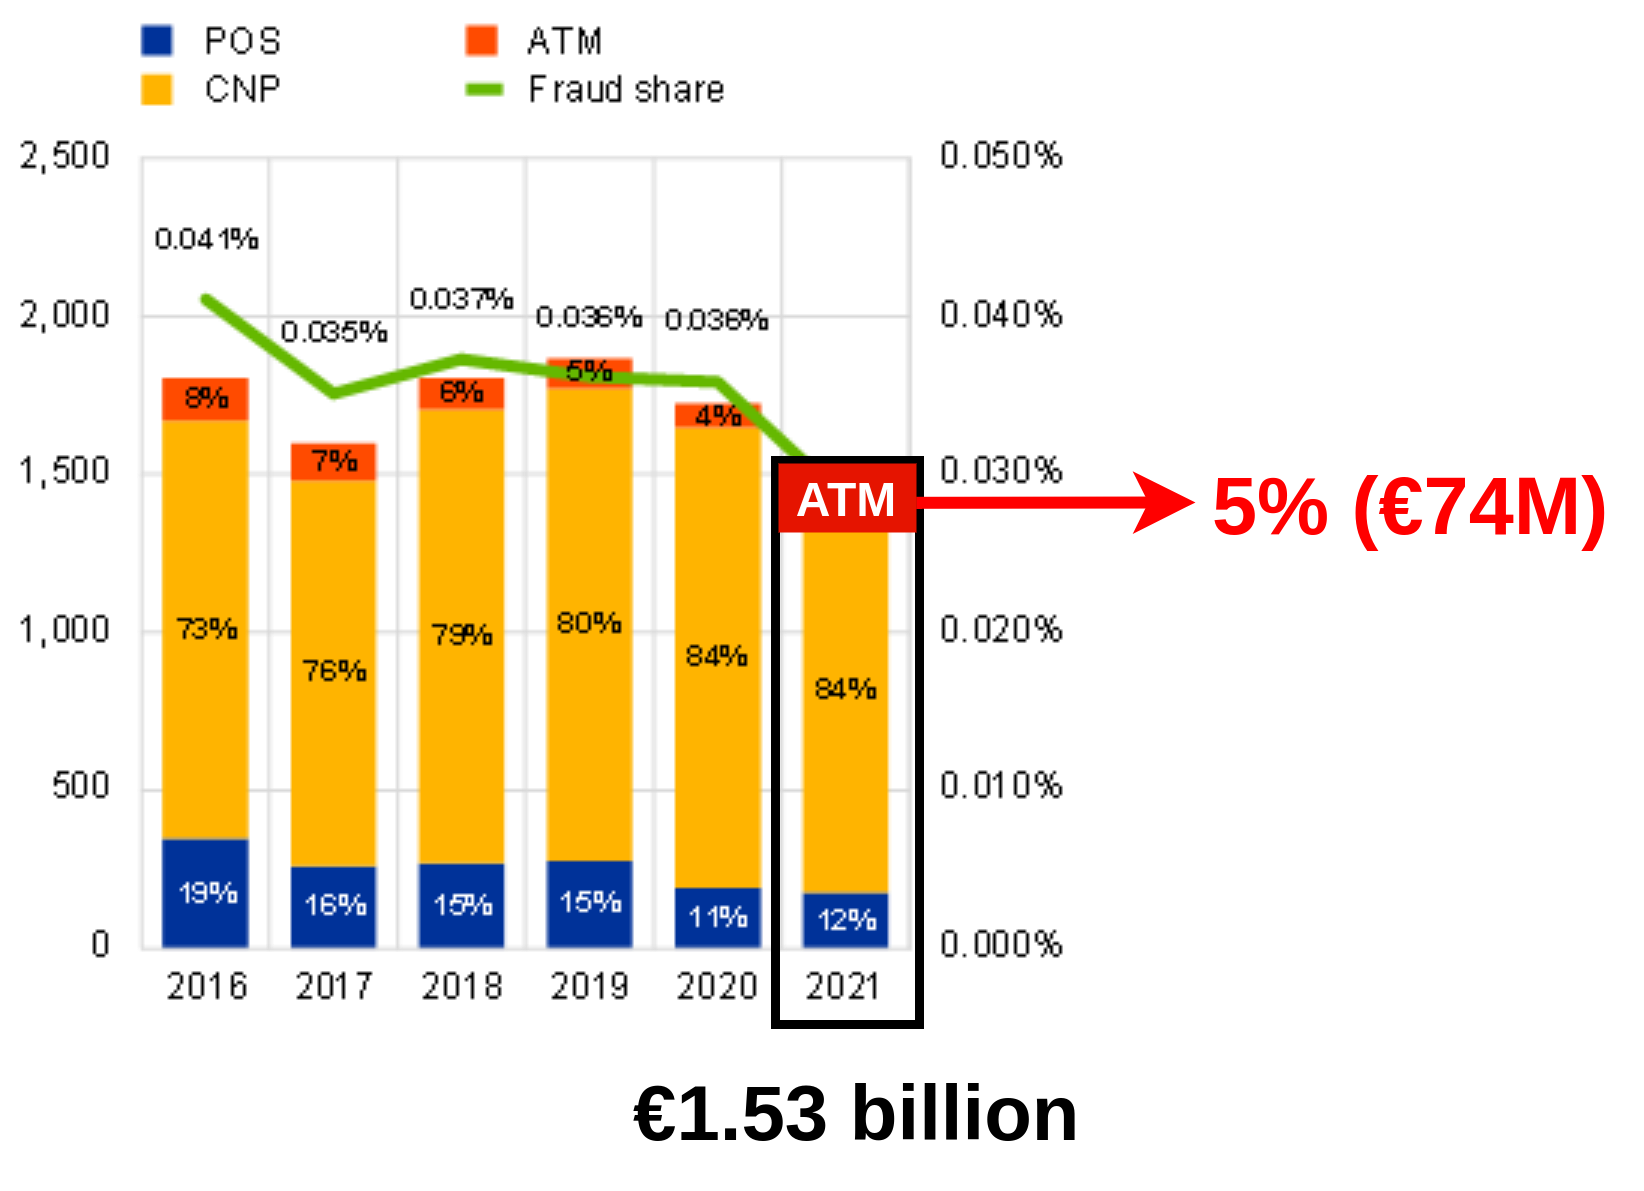
\includegraphics[width=0.8\linewidth]{figures/cardFraudTrends-2.png}
    \end{figure}
    %\begin{itemize}
    %    \item Card-Present (ATM and POS (Point-Of-Sale) terminals).
    %    \item Card-Not-Present (CNP). E.g. via the internet. 
    %\end{itemize}
    %\item Majority of card fraud related to CNP transactions.
    %\item In both 2020 and 2021, CNP fraud accounted for approximately 84\% of the total value of card fraud.
    %\item Card-present fraud committed at ATMs and POS terminals continued to decline in 2021 (-6.4\%), following a decrease of 27.7\% in the previous year. 
    %\item Value of ATM fraud $\sim$ €74M; POS terminals €177M (2021).
    %\item Losses from lost or stolen cards continued to be the main type of card-present fraud, accounting for 88\% of all ATM and 56\% of all POS fraud in 2021. 
    %\item The decrease in the value of ATM fraud in 2021 was driven by a further strong decline in counterfeit card fraud (-67.3\%), which only accounted for 3\% of total ATM fraud.
\end{itemize}
\end{frame}

%different artificial intelligence methods in terms of their accuracy (correct prediction of fraud) and claim that the accuracy is low in most of them.
\begin{frame}{Motivation: ATM Fraud Detection - State of the Art}
    \begin{itemize}
        \item \raisebox{-0.5em}{
\includegraphics[height=2em]{figures/classical-pic.png}} \textbf{Classical Treatment}:
        \vspace{0.5em}
        \begin{itemize}
            \item[\textcolor{red}{\ding{55}}] \textbf{Delayed} annoying consulting of \textbf{log files} because of customers complain when they themselves detect some weird movement in their accounts.
        \end{itemize}
        \vspace{0.4em}
        \item \raisebox{-0.5em}{
\includegraphics[height=2em]{figures/ML.png}} \textbf{ML Systems}:
        \vspace{0.5em}
        \begin{itemize}
            \item[\textcolor{red}{\ding{55}}] Detection based on \textbf{predictions}, not exact detection ($<$ 100\% accuracy).
            \vspace{0.3em}
            \item[\textcolor{red}{\ding{55}}] Need \textbf{training} process and big volumes of \textbf{data}.
            \vspace{0.3em}
            \item[\textcolor{red}{\ding{55}}] Quality of the predictions depends on the training data (possibly \textbf{biased}).
        \end{itemize}
    \end{itemize}
    \vspace{0.5em}
    $\rightarrow$ To our knowledge, most of the works are based on artificial intelligence techniques. No clear characterization of the problem. \cite{Rahman2019}.\\
\end{frame}

\begin{frame}{Motivation: ATM Fraud Detection}

We propose a system to overcome the previous problems:
\vspace{1em}
\begin{itemize}
    \item[\textcolor{green}{\ding{51}}] A \textbf{exact} detection of the fraud. \textbf{100\% accuracy}.
    \vspace{1em}
    \item[\textcolor{green}{\ding{51}}] In \textbf{real-time}.
    \vspace{1em}
    \item[\textcolor{green}{\ding{51}}] With a \textbf{clear characterization} of some fraud patterns.
    \vspace{1em}
    \item[\textcolor{green}{\ding{51}}] A synthetic \textbf{bank dataset} and \textbf{transaction stream generator tool} (lack of real-world data). % Lack of real-world data due to the sensitive nature of banking data and transactions.  
\end{itemize}
\end{frame}

\begin{comment}
\begin{frame}{Contributions}
\begin{itemize}
\item A \textbf{Continuous Query Engine} to detect abnormal or suspicious ATM transactions in \textbf{real-time}, with \textbf{100\% accuracy: $\mathsf{DP_{ATM}}$}
\vspace{1em}
\pause
\item A \textbf{characterization} of some possible \textbf{fraud} (graph) \textbf{patterns}.
\vspace{1em}
\pause
%Even non-exhaustive, to our knowledge, it is a first specification of what must be consider a fraud pattern in terms of (continuous) graph databases. This characterization is useful not only when considering ATM transactions but, in general,  for any bank cards online transactions.
\item A general technique for addressing the problem of \textbf{continuous 
query evaluation} against an \textbf{evolving graph database}.
% by decomposing the data graph into \emph{volatile} and \emph{stable} well defined subgraphs, using a stream processing approach.  
\vspace{1em}
\pause
\item A synthetic \textbf{bank dataset} and \textbf{transaction stream generator tool} (lack of real-world data). % Lack of real-world data due to the sensitive nature of banking data and transactions. 
\end{itemize}
\end{frame}
\end{comment}

\begin{comment}
\begin{frame}{Motivation: Example (I)}

\begin{figure}
    \hspace*{-0.5cm} % adjust the value to control the leftward shift
    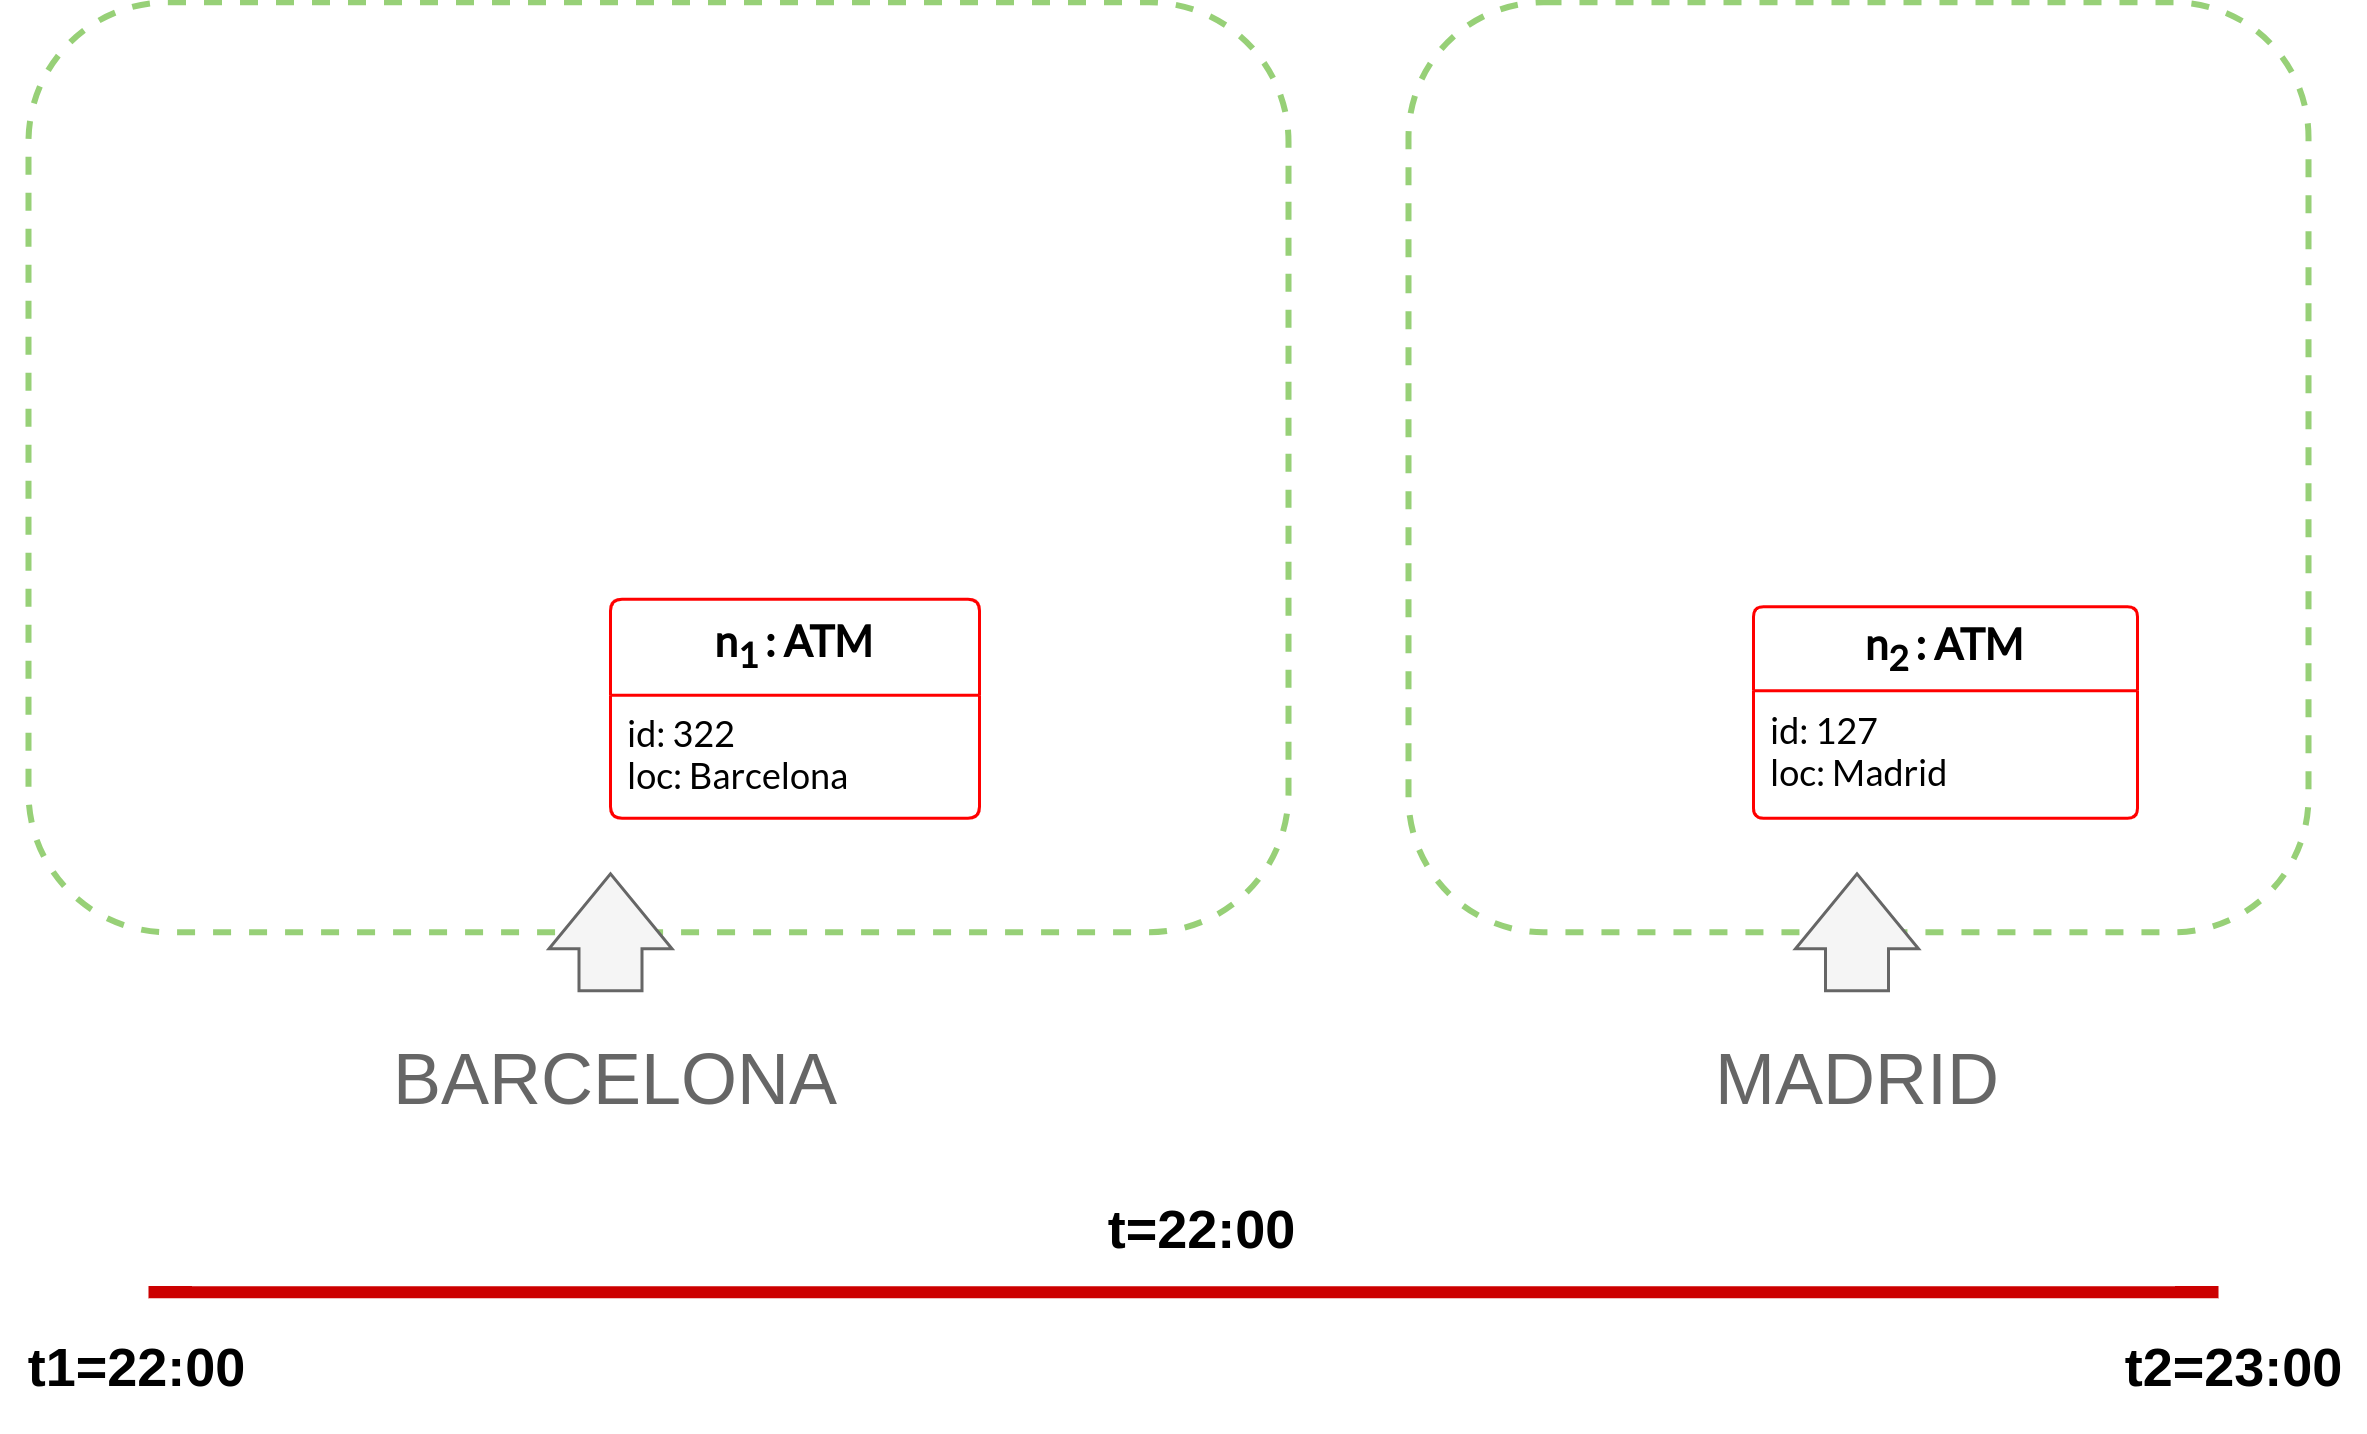
\includegraphics[width=1.1\textwidth]{figures/sequenceExample-1.png}
\end{figure}

\end{frame}

\begin{frame}{Motivation: Example (II)}

\begin{figure}
    \hspace*{-0.5cm} % adjust the value to control the leftward shift
    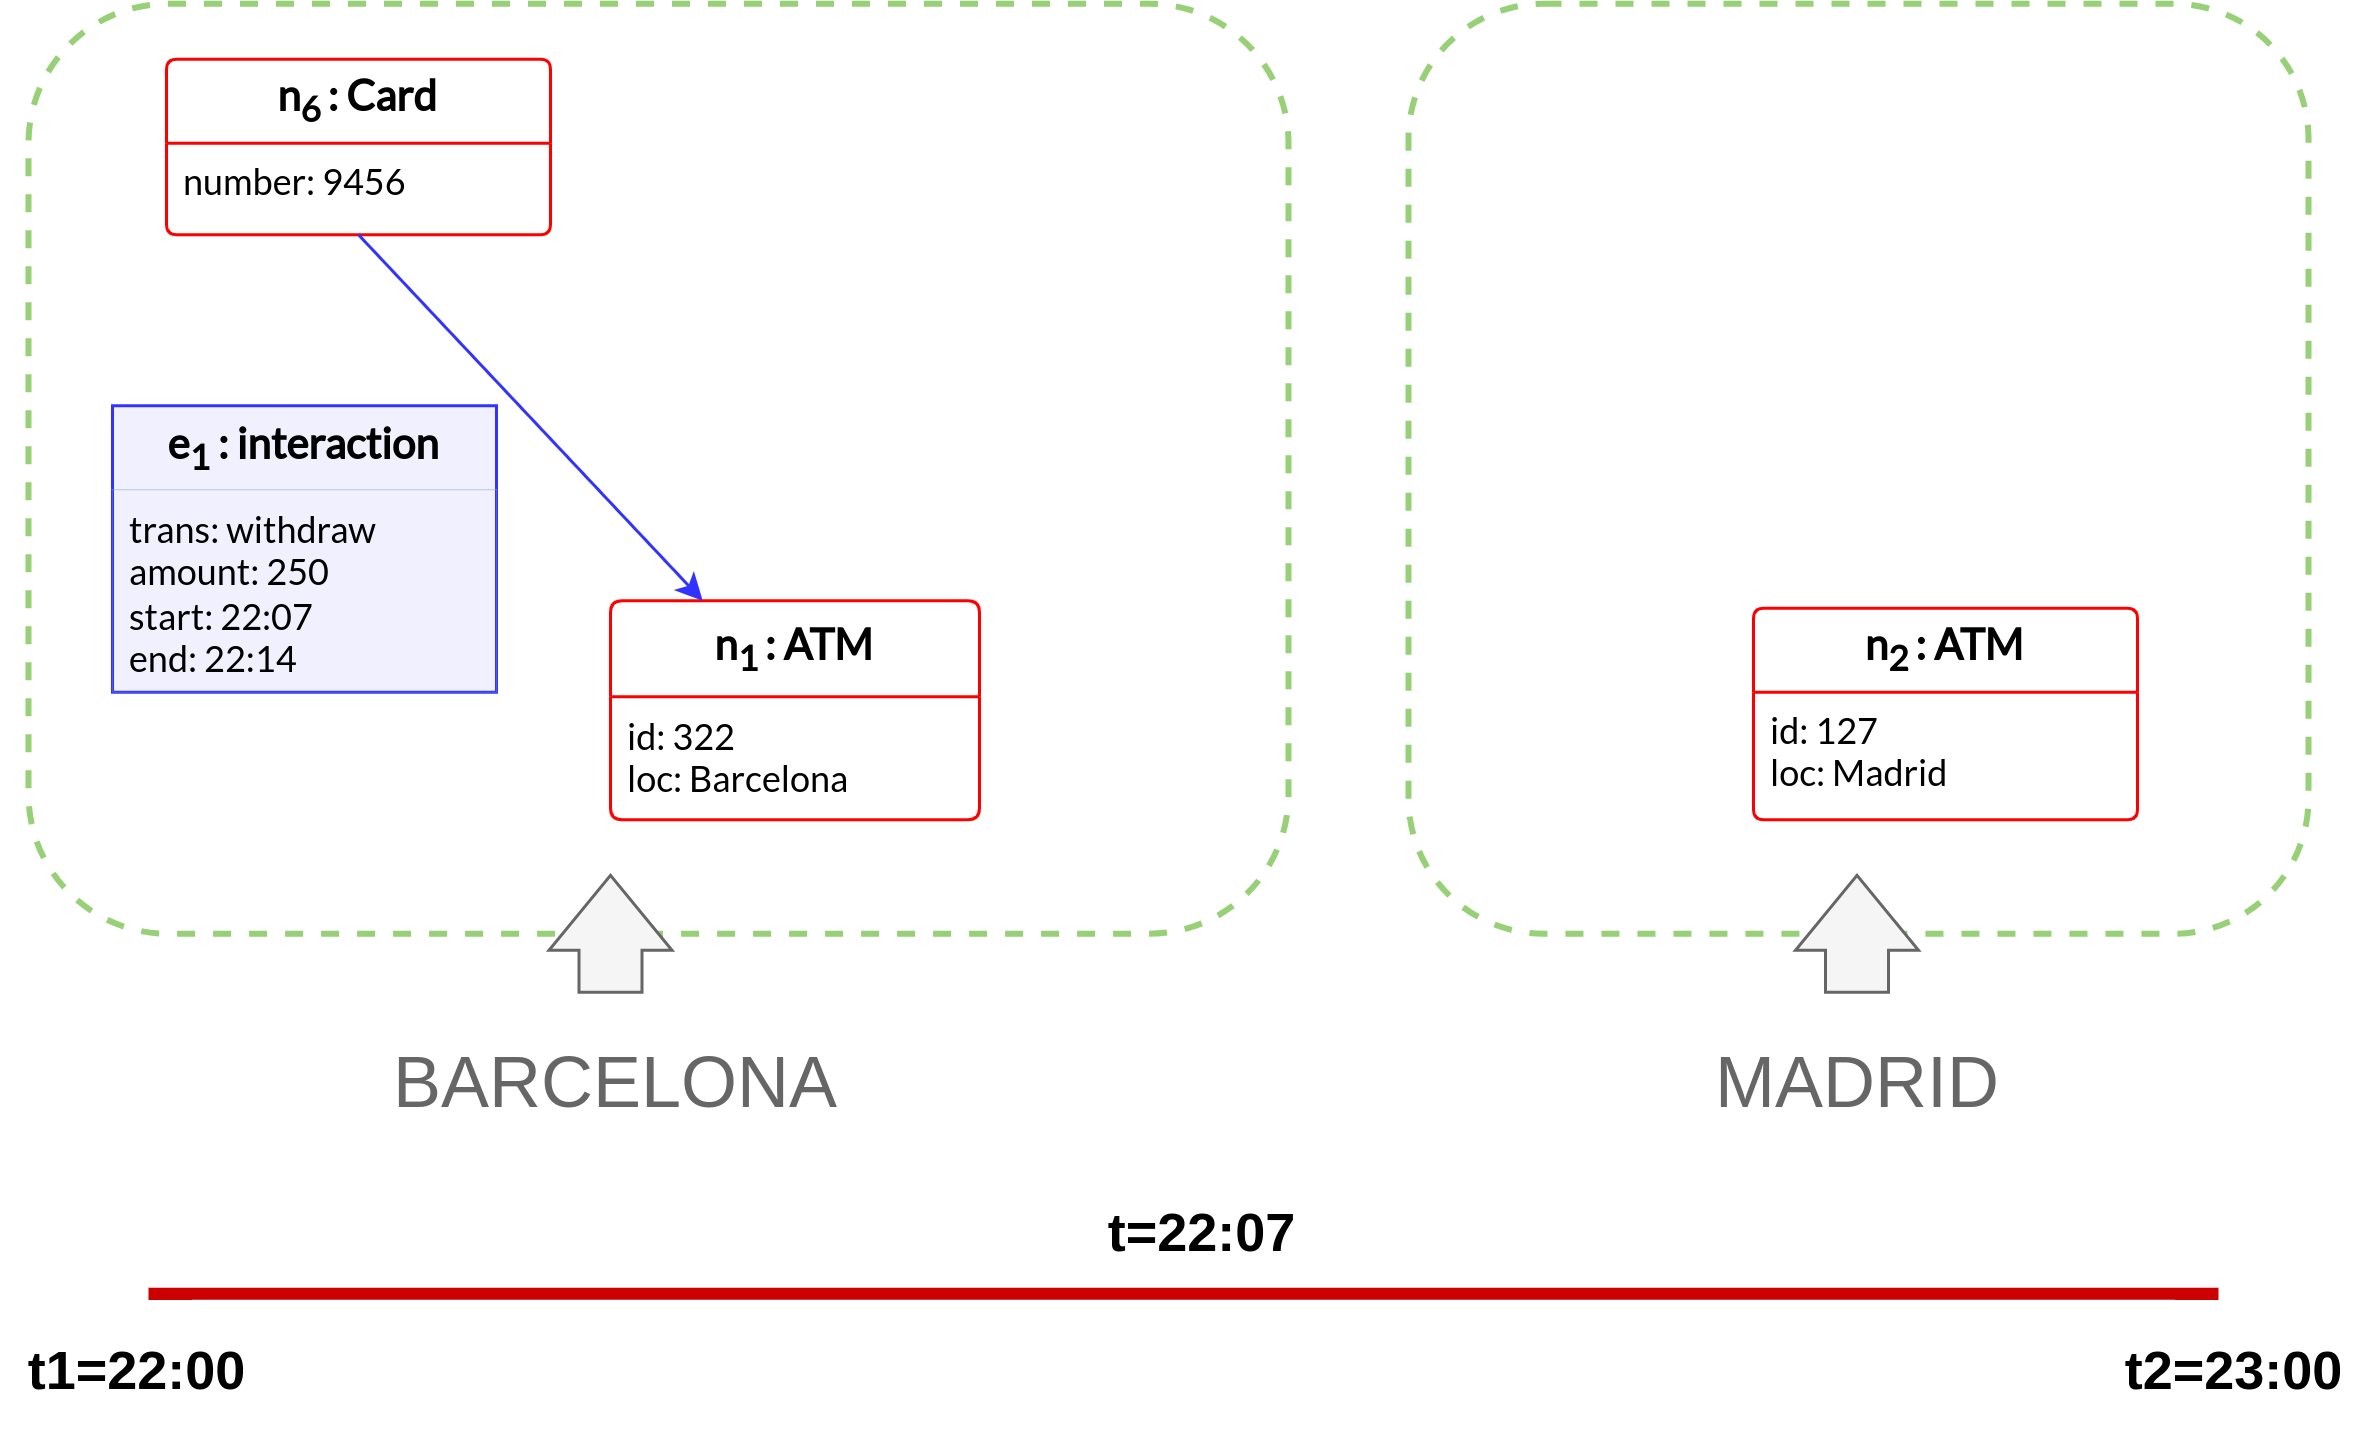
\includegraphics[width=1.1\textwidth]{figures/sequenceExample-2.png}
\end{figure}

\end{frame}

\begin{frame}{Motivation: Example (III)}

\begin{figure}
    \hspace*{-0.5cm} % adjust the value to control the leftward shift
    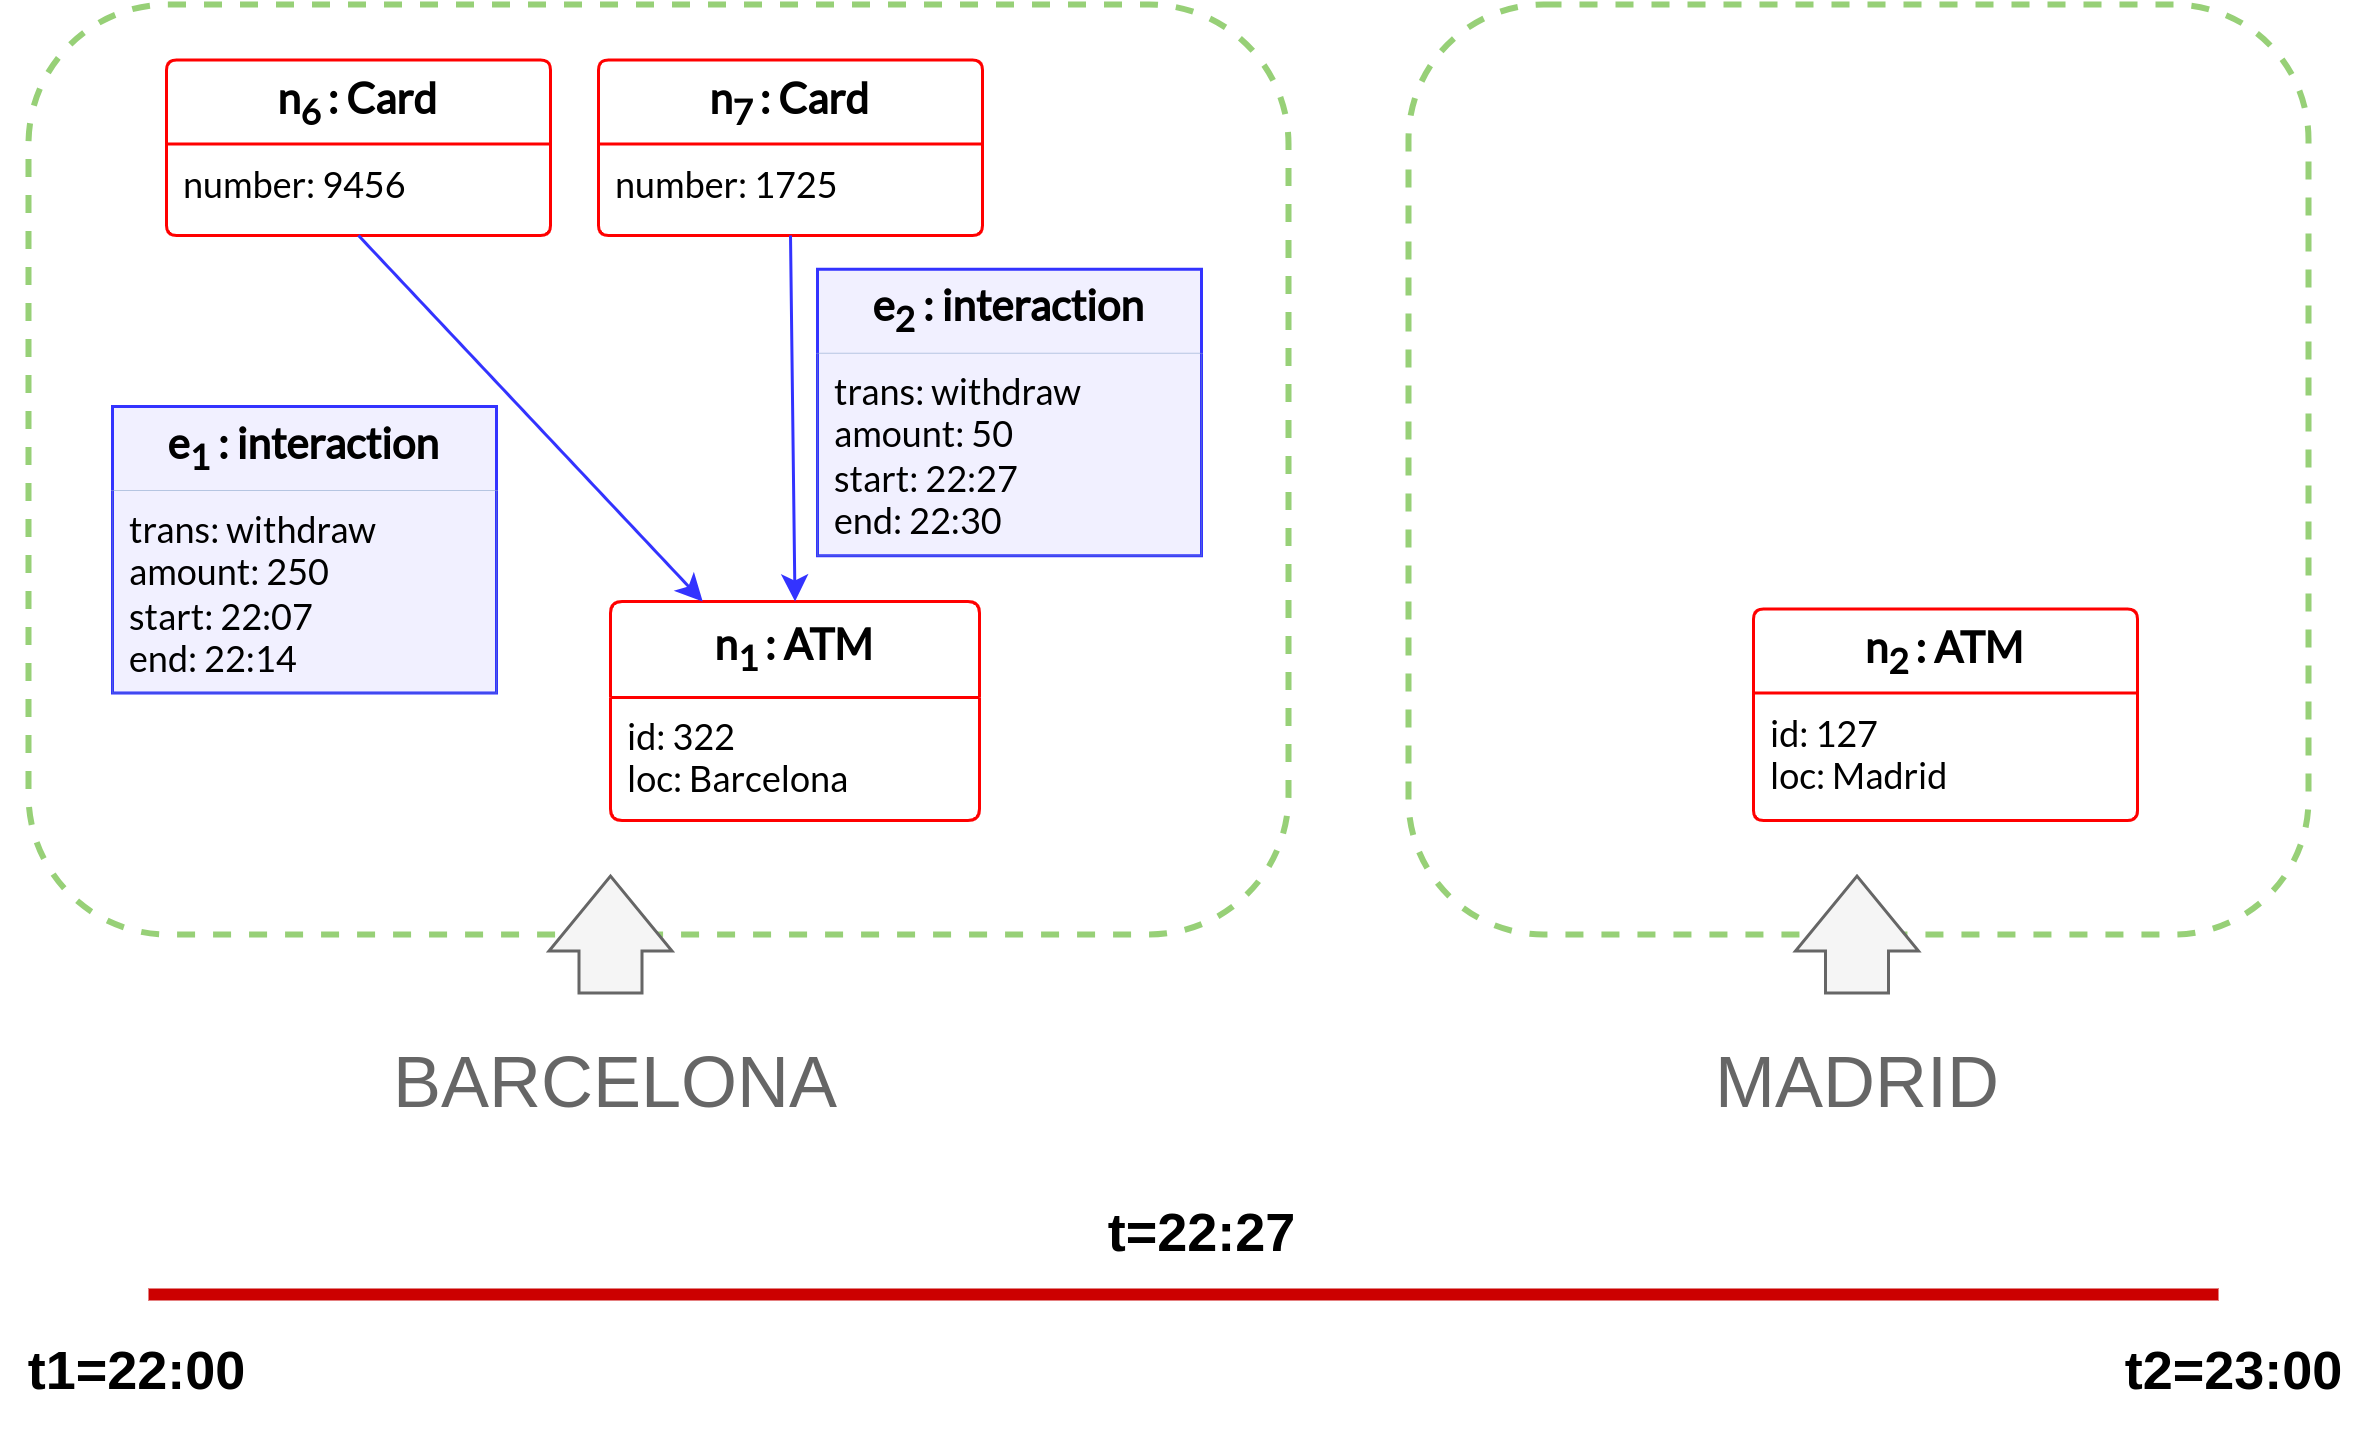
\includegraphics[width=1.1\textwidth]{figures/sequenceExample-3.png}
\end{figure}

\end{frame}

\begin{frame}{Motivation: Example (IV)}

\begin{figure}
    \hspace*{-0.5cm} % adjust the value to control the leftward shift
    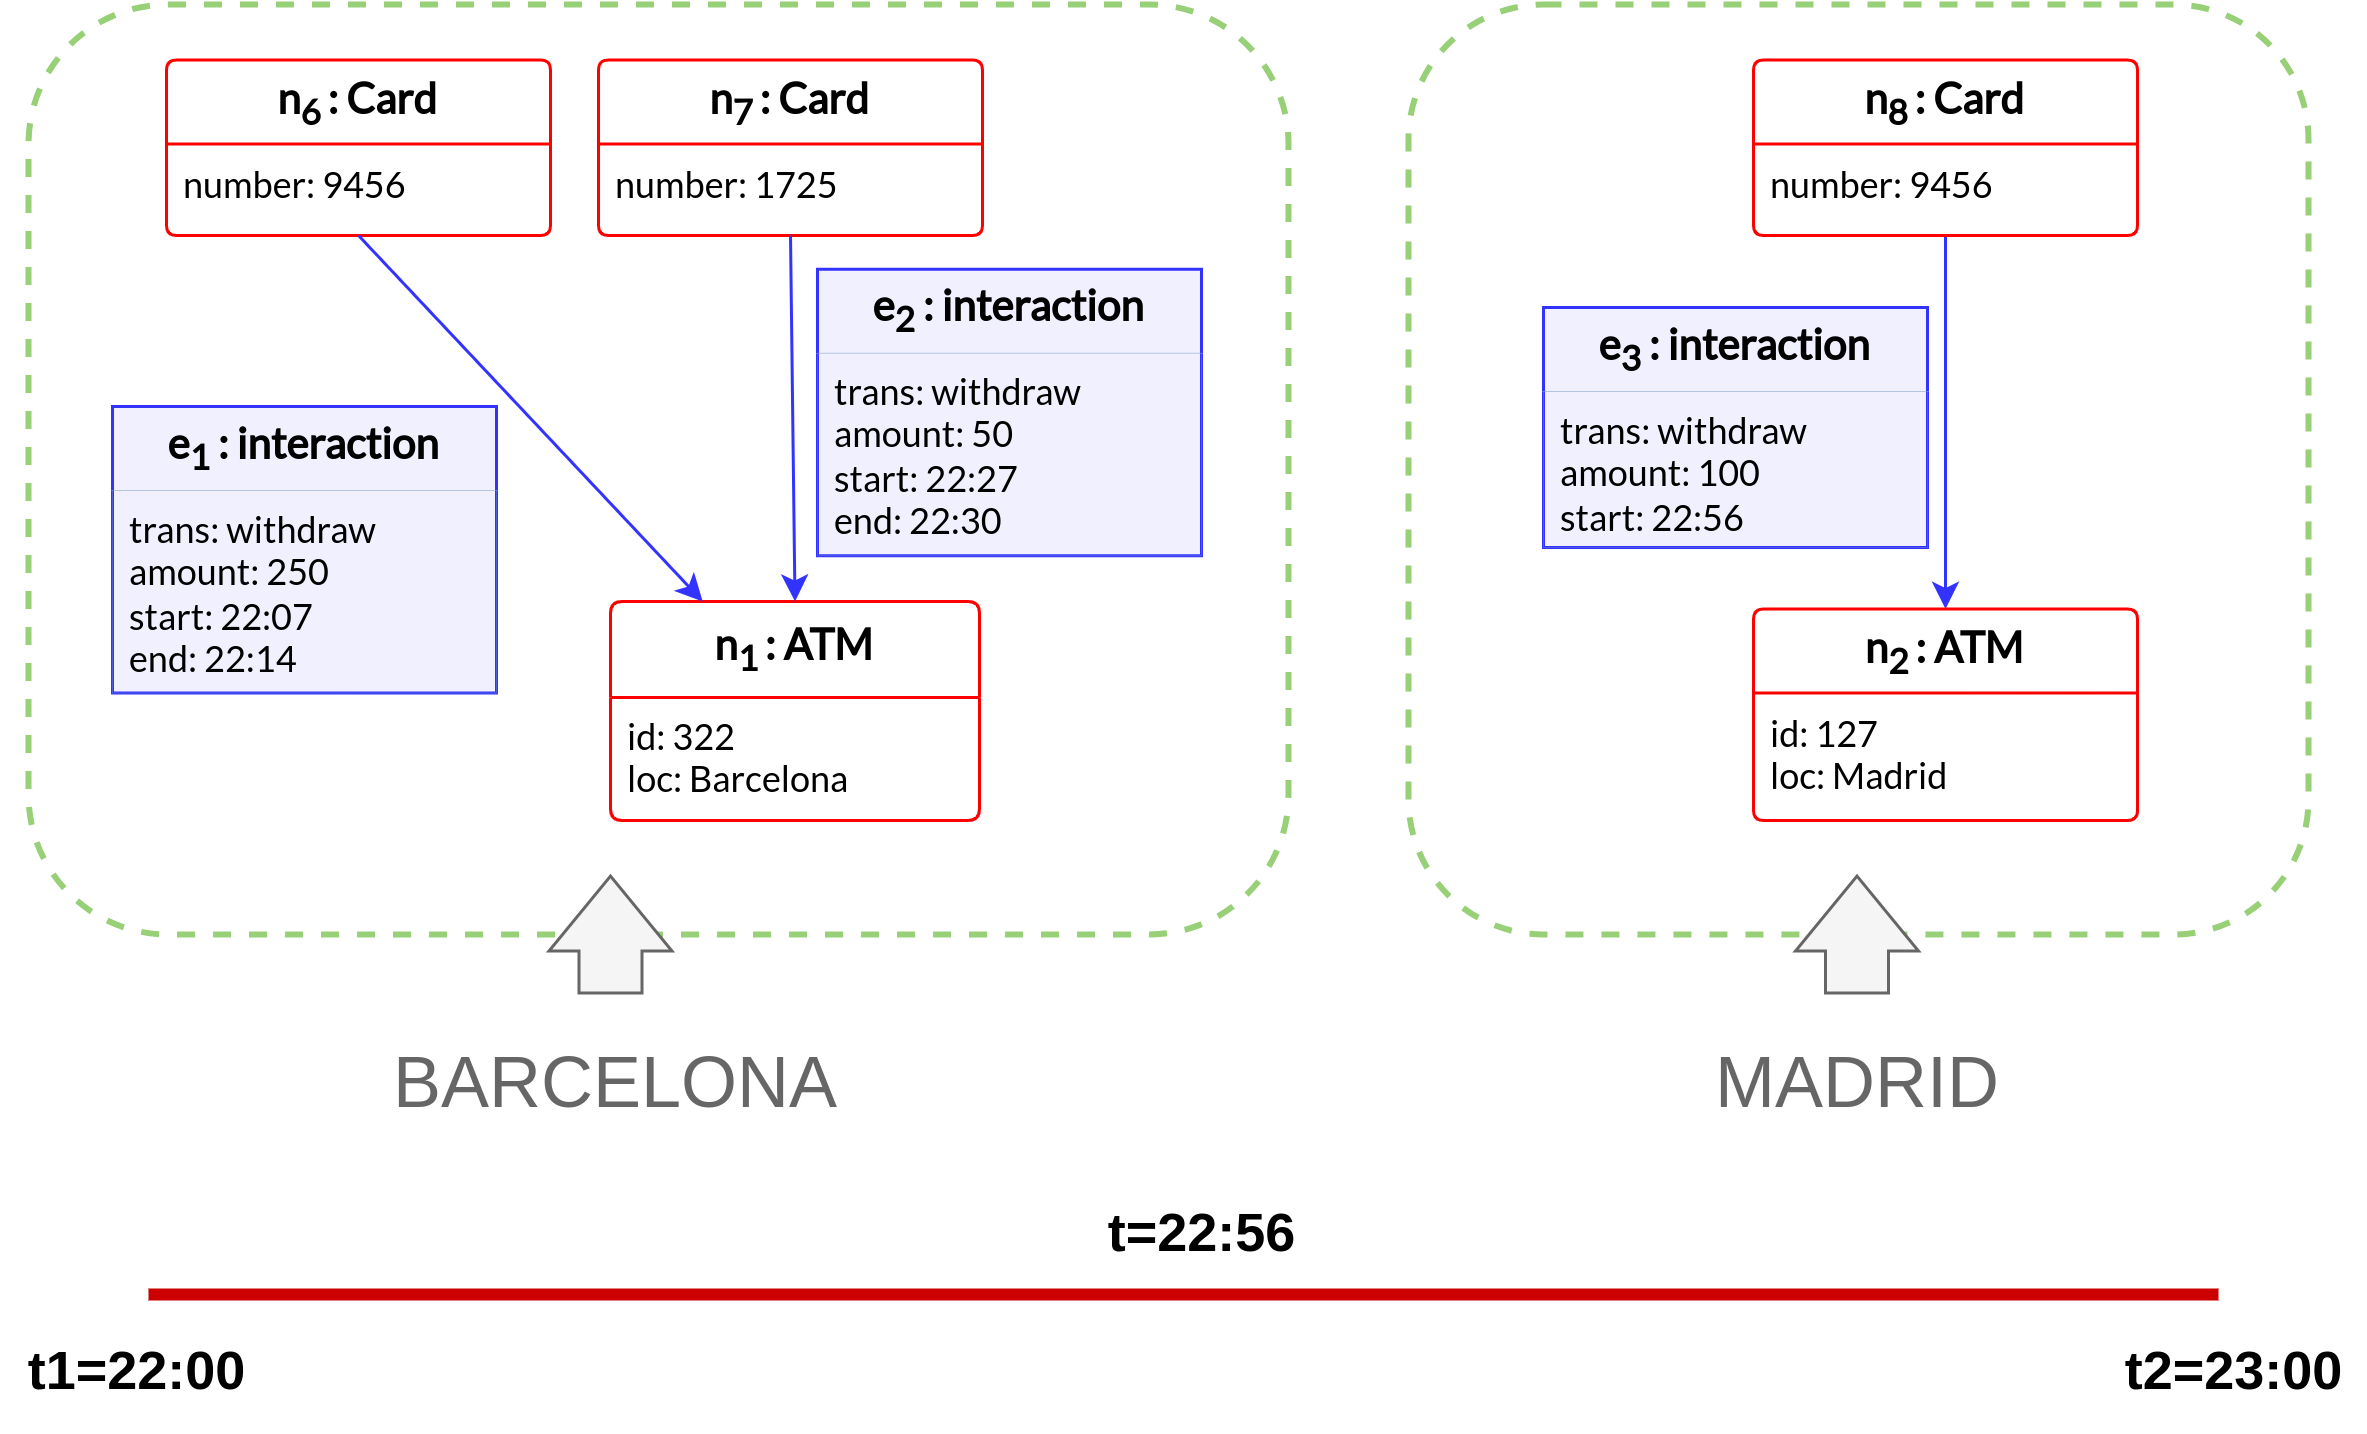
\includegraphics[width=1.1\textwidth]{figures/sequenceExample-4.png}
\end{figure}

\end{frame}

\begin{frame}{Motivation: Example (V)}

\begin{figure}
    \hspace*{-0.5cm} % adjust the value to control the leftward shift
    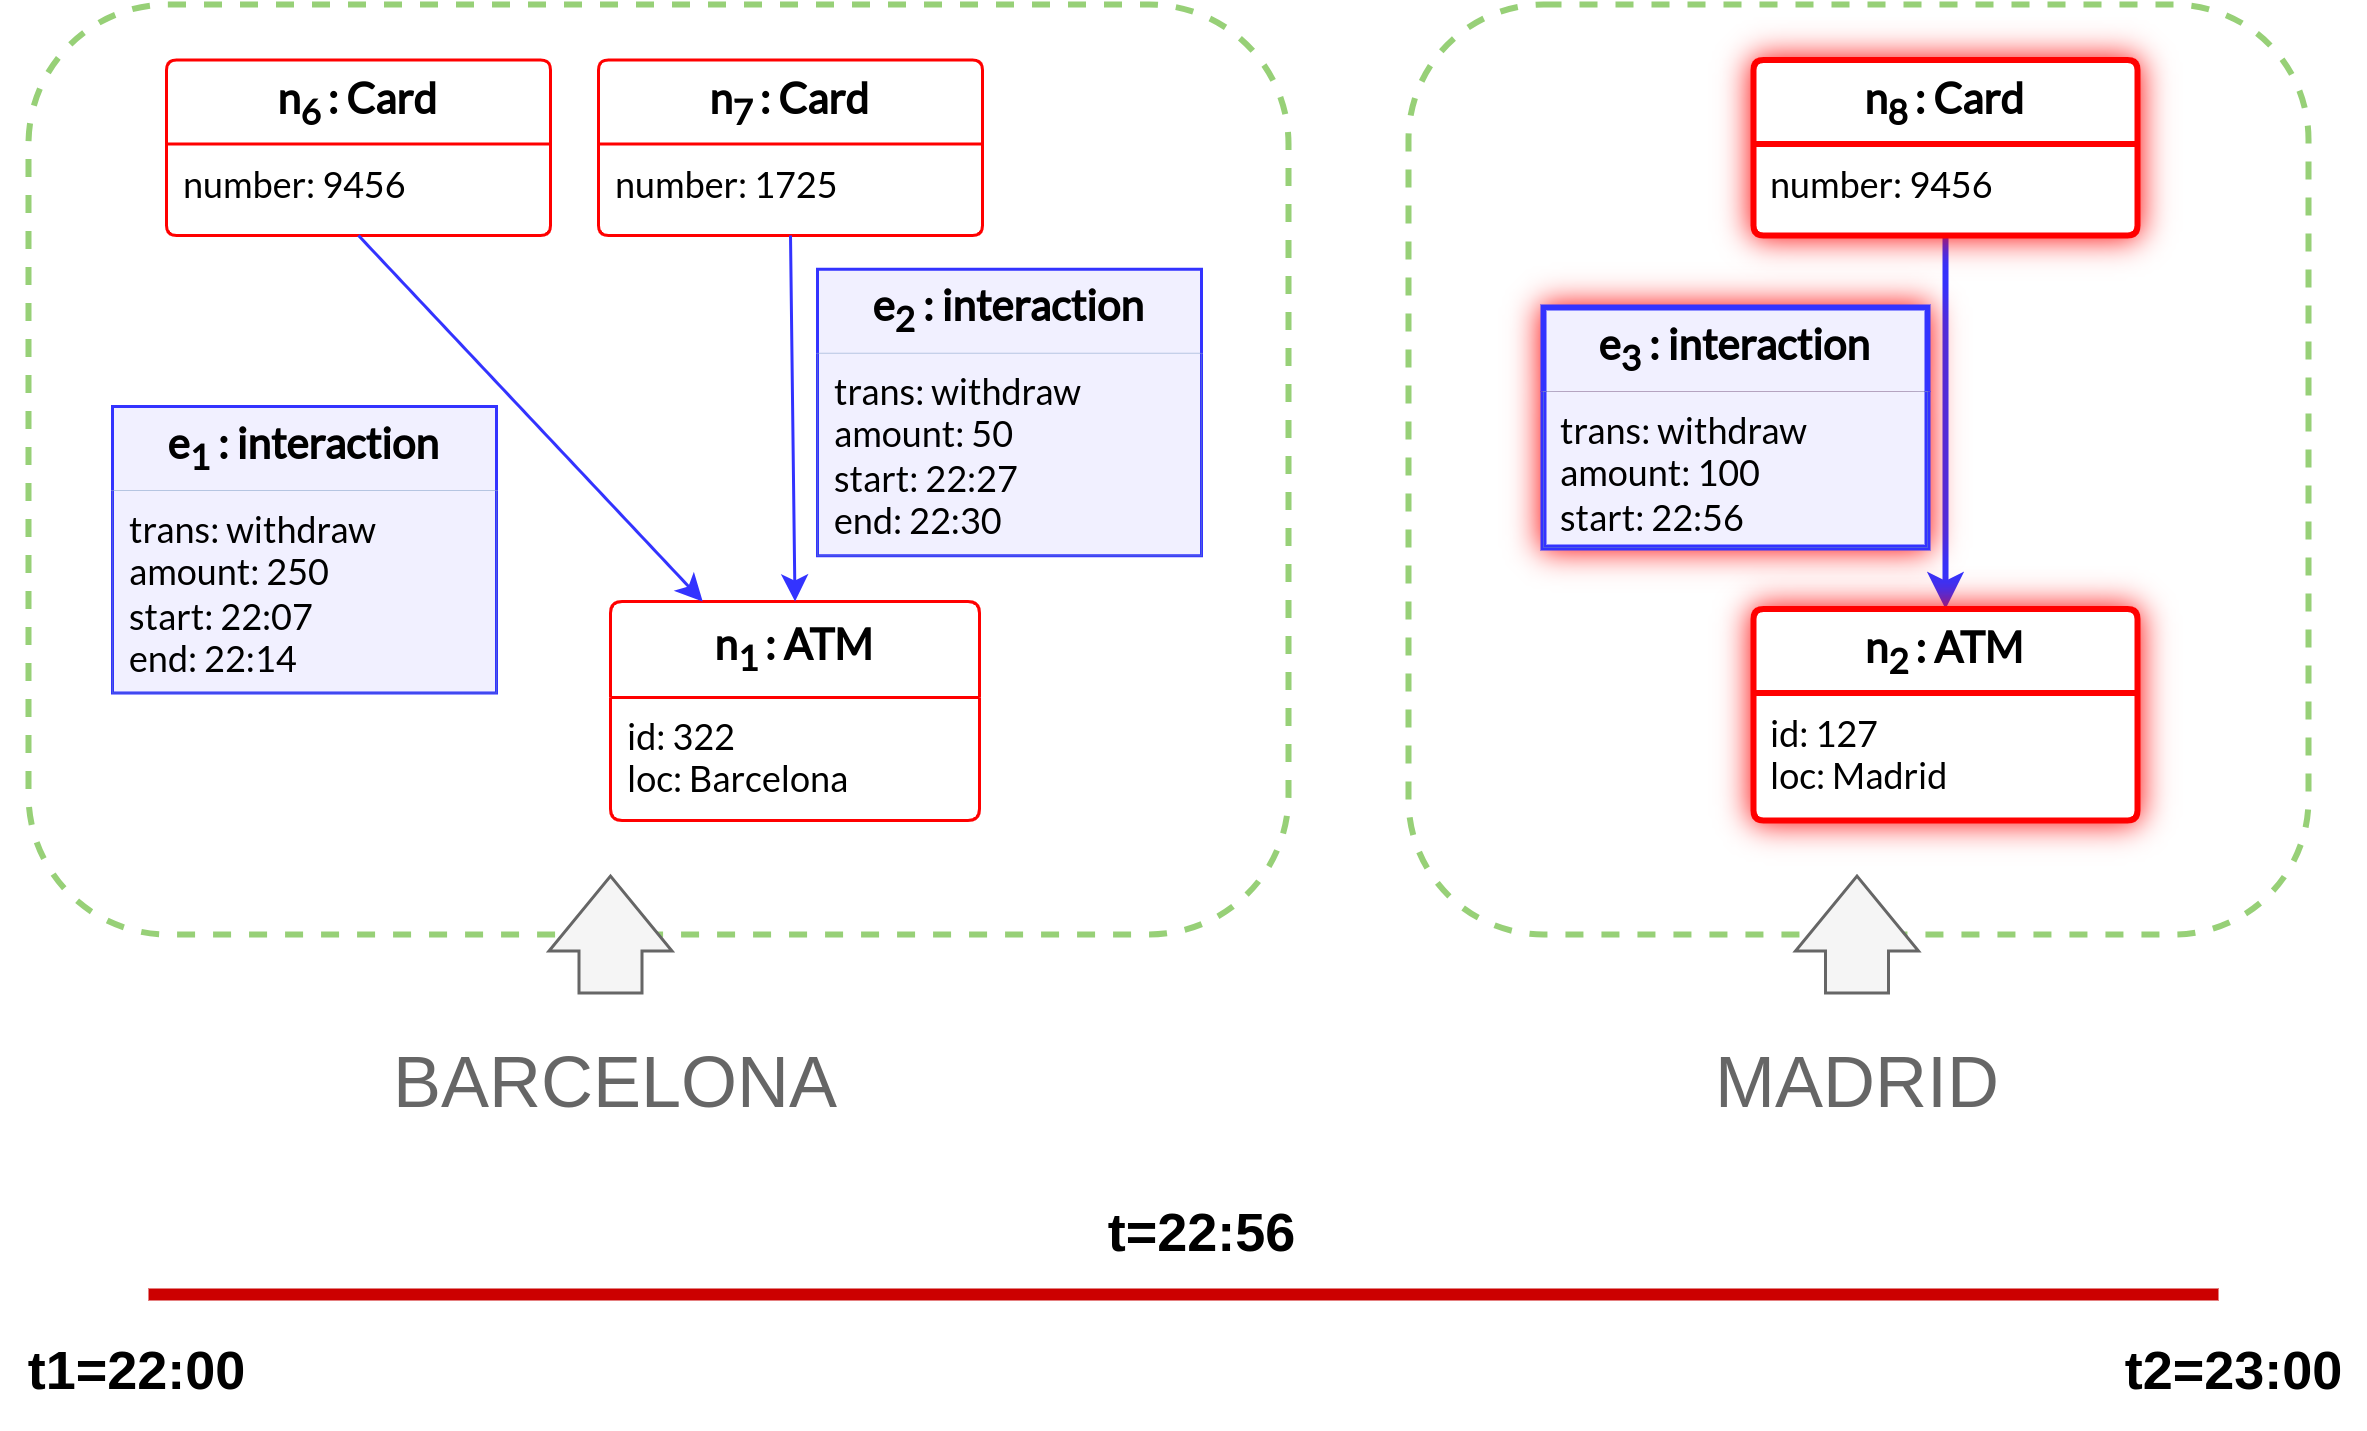
\includegraphics[width=1.1\textwidth]{figures/sequenceExample-5.png}
\end{figure}

\end{frame}

\begin{frame}{Motivation: Example (V)}

\begin{figure}
    \hspace*{-0.5cm} % adjust the value to control the leftward shift
    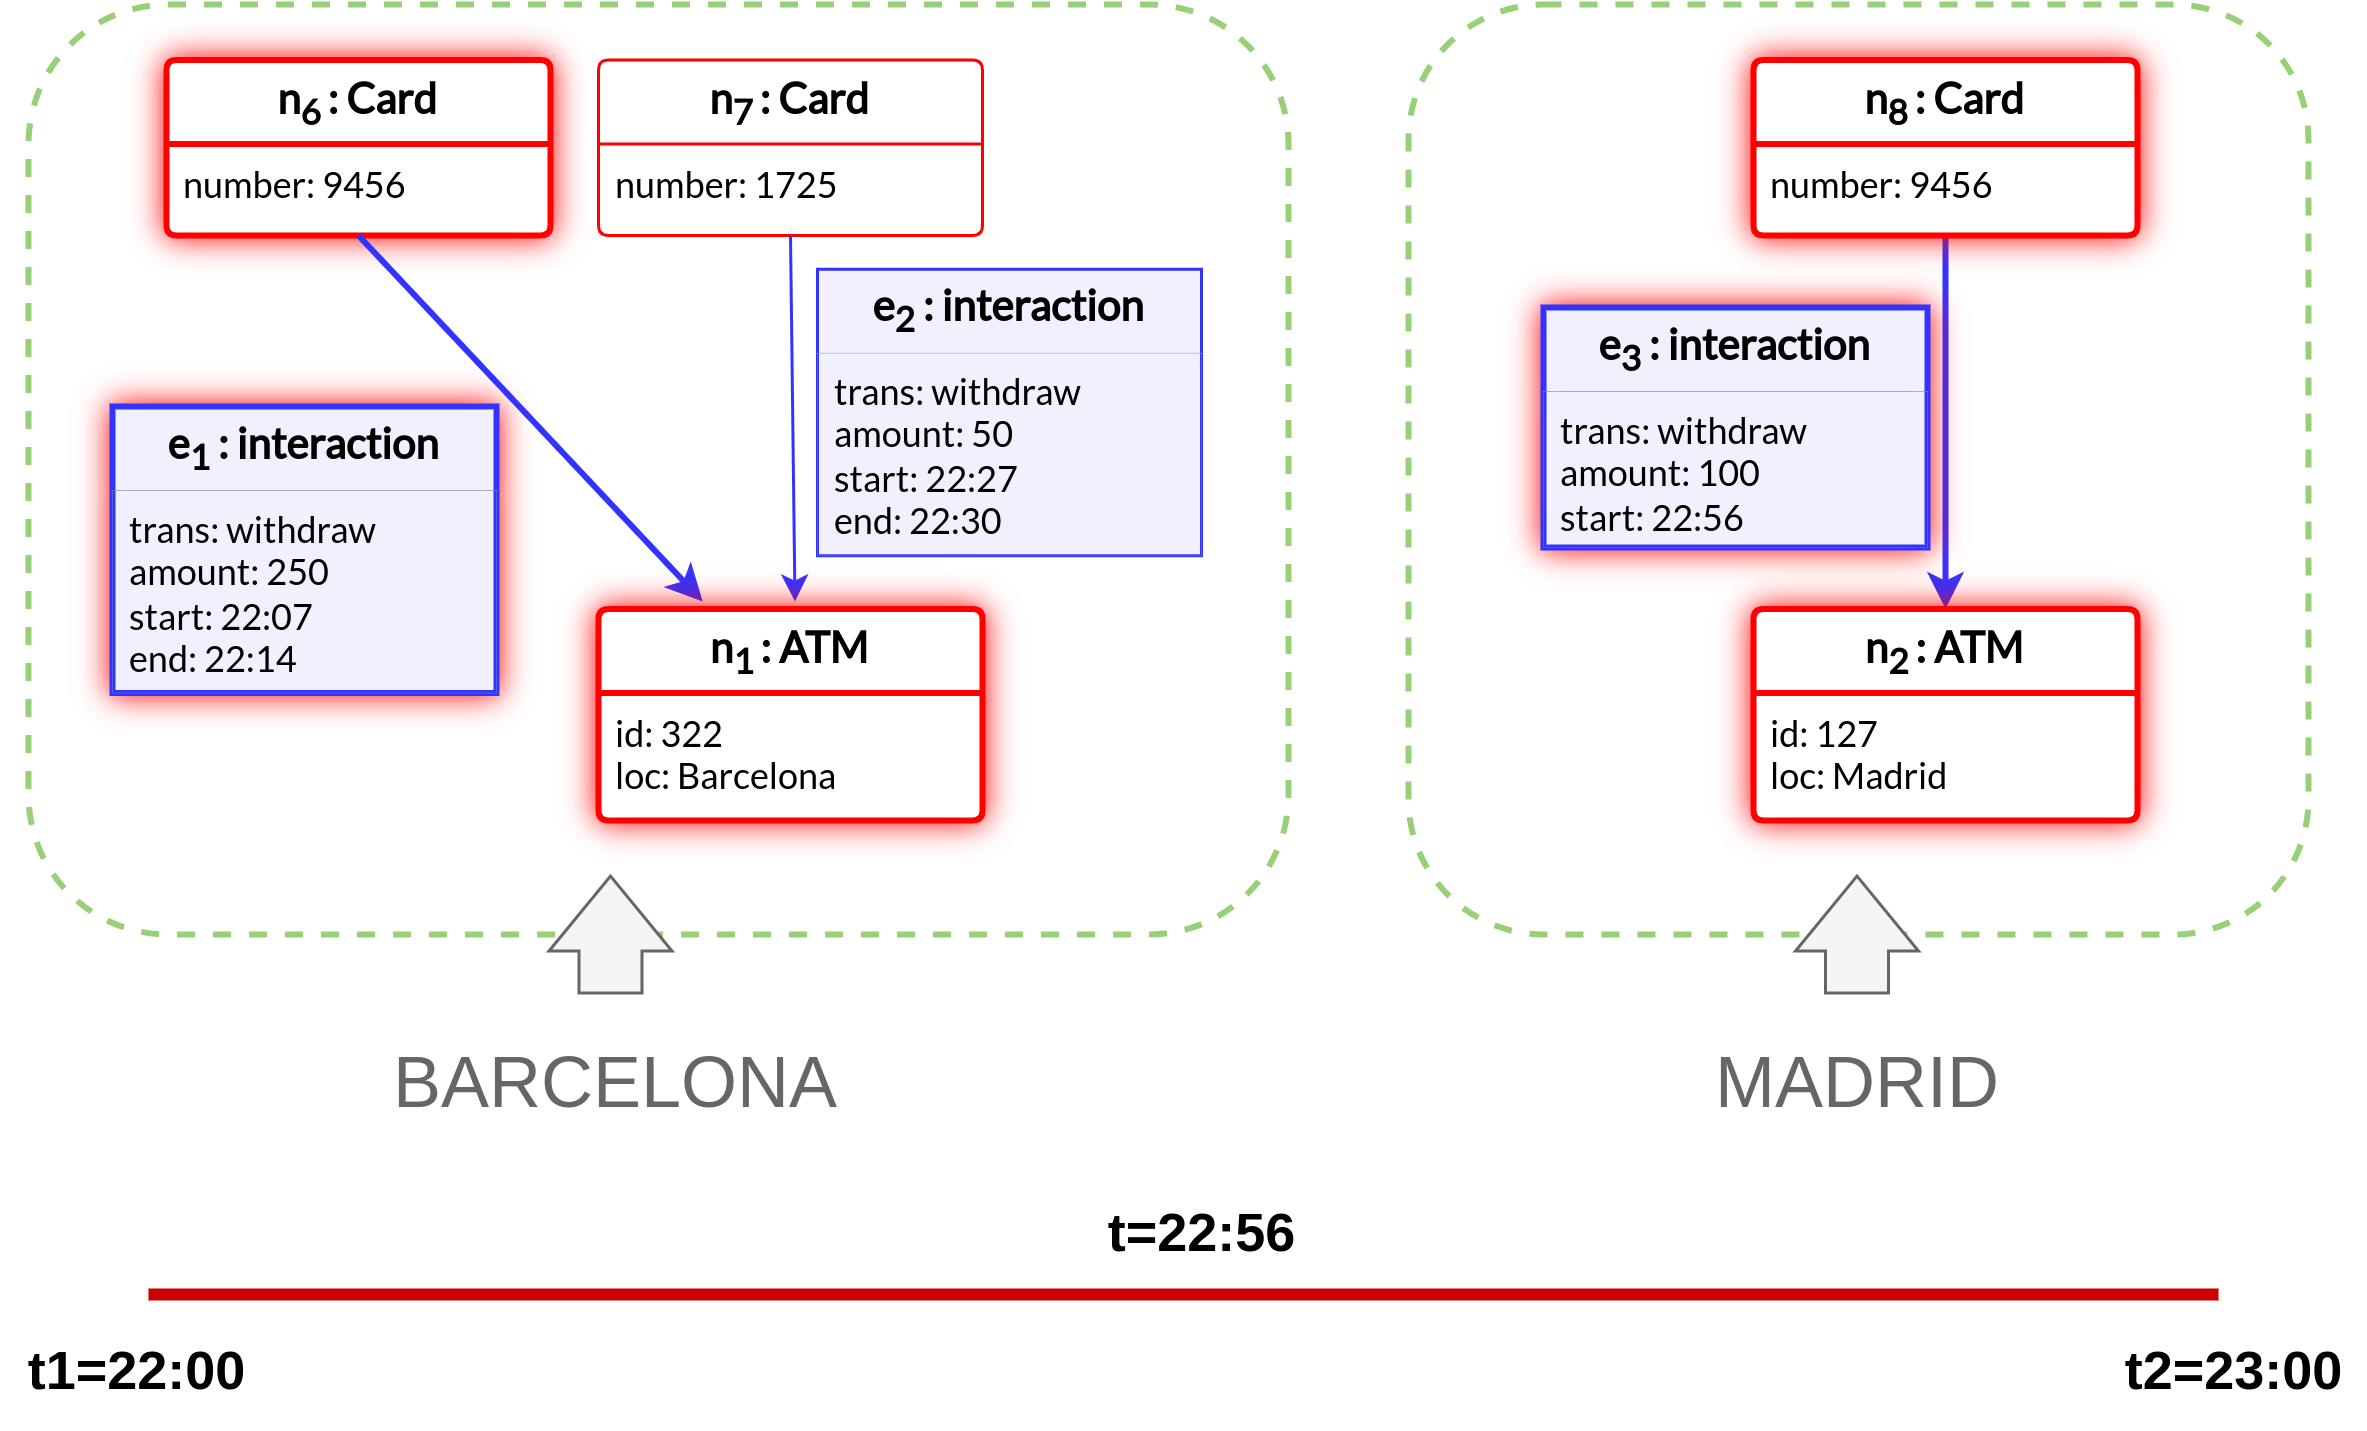
\includegraphics[width=1.1\textwidth]{figures/sequenceExample-5-1.png}
\end{figure}

\end{frame}


\begin{frame}{Motivation}

\begin{figure}
    \hspace*{-0.5cm} % adjust the value to control the leftward shift
    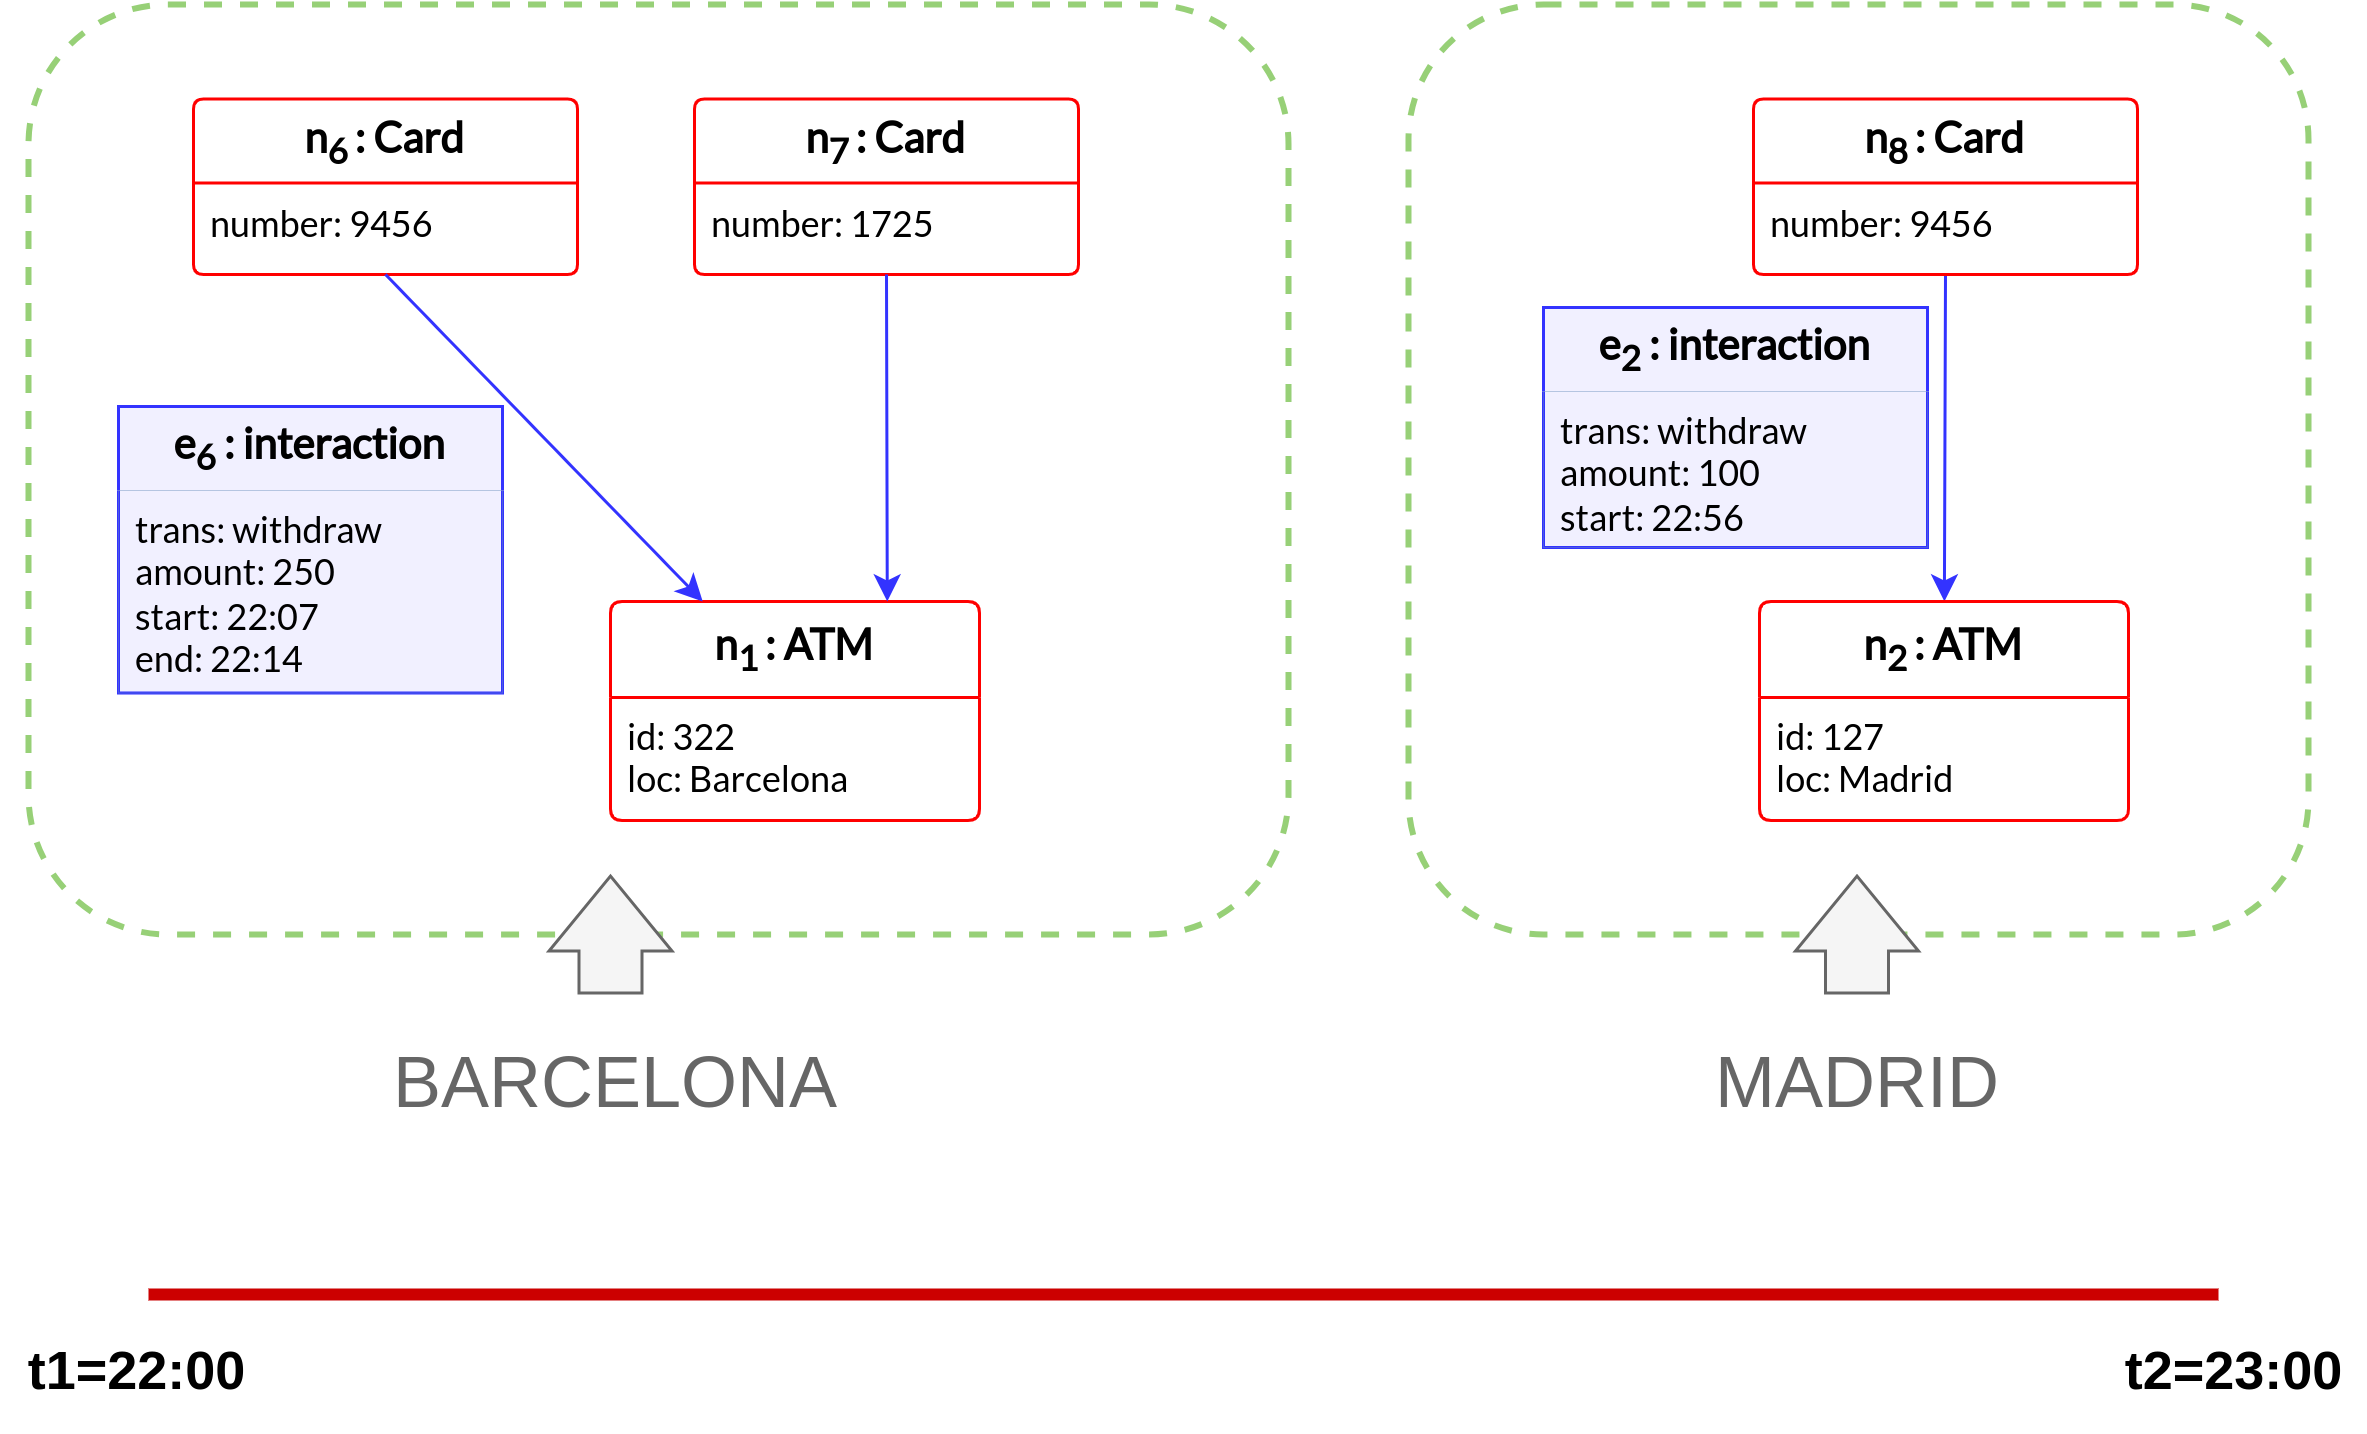
\includegraphics[width=1.1\textwidth]{figures/sequenceExample.png}
\end{figure}

\end{frame}

\begin{frame}{Motivation}

\begin{figure}
    \hspace*{-1cm} % adjust the value to control the leftward shift
    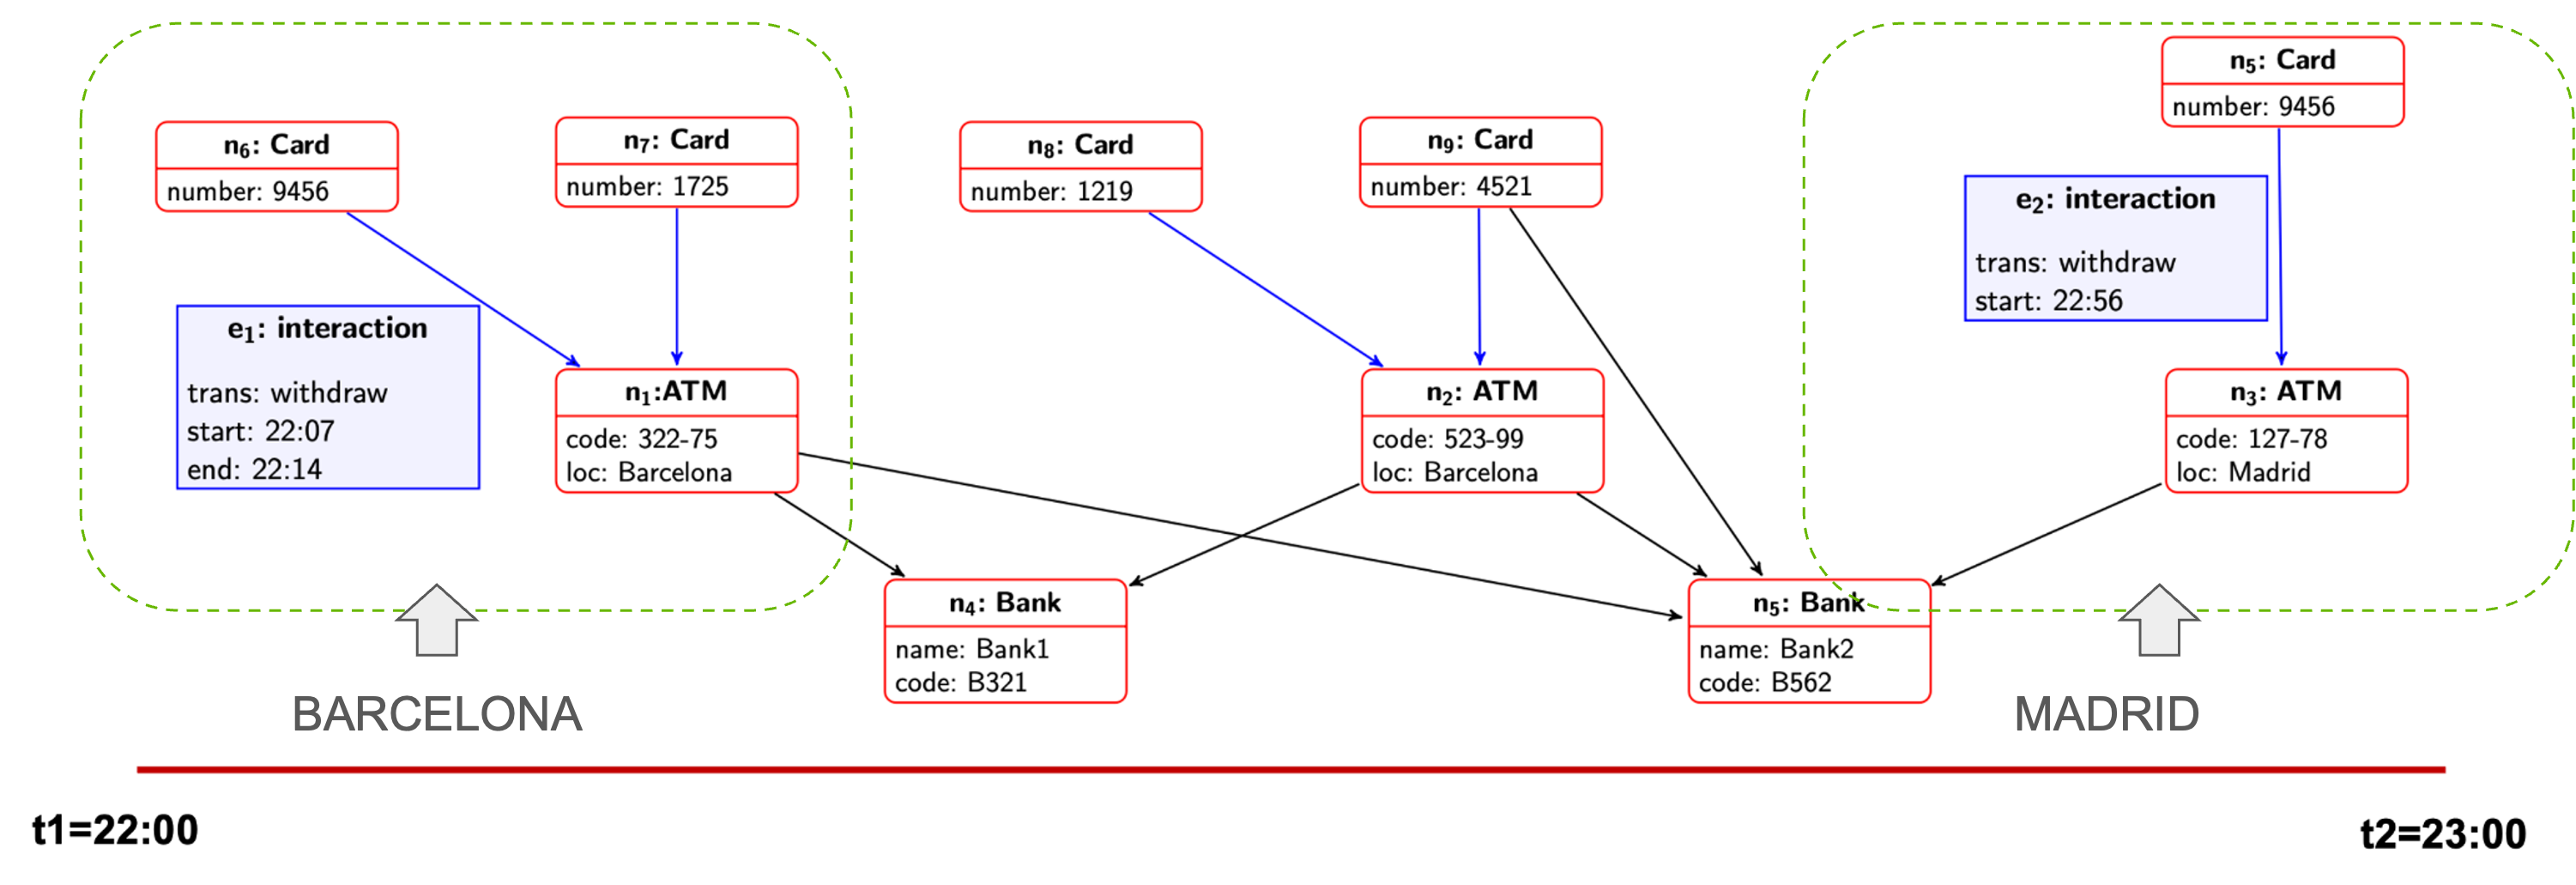
\includegraphics[width=1.1\textwidth]{figures/theProblem.png}
\end{figure}

\end{frame}

\begin{frame}{Motivation} \justifying

A system to detect anomalous patterns of ATM transactions against a continuously evolving PG representing a bank database.
\vspace{1cm}
\begin{itemize}
    \item (Massive) stream of transactions.
    \item On-the-fly emission of anomalous patterns alerts.
\end{itemize}
\end{frame}
\end{comment}

\begin{comment} 
In this work, as a proof of concept, we
tackled the problem of evaluating continuous queries corresponding to anomalous patterns
of ATM transactions against a continuously evolving PG representing a bank database. To
be concrete, the anomalous patterns of ATM transactions are identified in the volatile (PG)
subgraph of the considered database. The evaluation process is based on the dynamic pipeline
computational model and emits answers (alarms) as soon as anomalous patterns are identified.
Additionally, a log of all the volatile relations of the PG is maintained. Figure 2 illustrates a
possible anomalous situation associated to this query.
\end{comment}